\section{Initial thirteen-loop grid and the basis correction}
\label{sec:blocks13-initial}
The initial application combined earlier checked preferred master lists into one list per structure. This list could contain alternative basis elements. Different seed regions could then produce different master representations. A failed entrywise coefficient comparison therefore remains unverified; it is not treated as proof that the integral identity is wrong. The corrected application forms one basis by reducing the complete earlier index list on development parameters, checks it independently, and tests new physical profiles. No initial reserved coefficient enters model fitting or basis calibration.

The initial grid uses six coupled-family definitions at each loop order, with the stated one-loop omissions, and three additional scattering structures. It adds four product structures per loop order. Product blocks have at most two loops, share external kinematics, and use distinct loop momenta. An odd loop count adds a one-loop remainder. Unused cross-block scalar-product coordinates have zero target powers. An explicit structural check confirms that an active cross-block numerator joins its blocks.

The 52 product requests use rational profile $h=1307+4L$. The corrected products use $h=1607+4L$. The coupled profiles are 1301 and 1601, and the basis-calibration profile is 1501. The one-mass formula checks use $h=1409+6L$, and the massless numerator checks use $h=1801+6L$. The family equations and parameter rules follow Appendix~\ref{app:families-new}. The scalar vacuum checks raise one massless or the massive denominator by two powers; the numerator checks add one power to one denominator and insert one auxiliary quadratic numerator. Additional three- and four-loop checks use $(2k_1-3k_2+k_3)^2$ as the numerator. The massless checks raise one physical power and include both internal-momentum and external-momentum numerator coordinates. All stated dimension dependence remains symbolic.

\begin{table}[!htbp]\centering\small
\caption{Initial grid: three exactly checked completions and requested totals. These counts retain the basis mismatch and native resource limits.}
\begin{tabular}{rrrrr}\toprule
Loops & Requests & Native & Fixed & Learned\\\midrule
1 & 10 & 10 & 10 & 10\\
2 & 11 & 11 & 10 & 10\\
3 & 10 & 9 & 6 & 6\\
4 & 10 & 8 & 7 & 7\\
5 & 10 & 6 & 5 & 5\\
6 & 10 & 5 & 4 & 4\\
7 & 10 & 5 & 4 & 4\\
8 & 10 & 4 & 3 & 3\\
9 & 10 & 5 & 4 & 4\\
10 & 10 & 4 & 3 & 3\\
11 & 10 & 5 & 4 & 4\\
12 & 10 & 4 & 3 & 3\\
13 & 10 & 5 & 4 & 4\\
\bottomrule\end{tabular}\end{table}
\begin{figure}[!htbp]\centering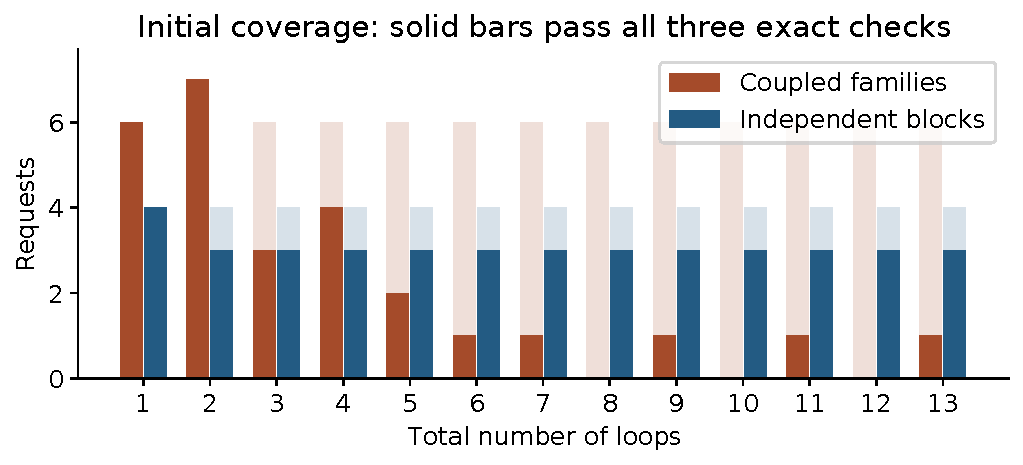
\includegraphics[width=.9\linewidth]{paper_figures/factorized_coverage.pdf}
\caption{Initial grid coverage. Pale bars show requested cases and solid bars show three checked learned completions. Independent products and coupled families have different native requirements.}\end{figure}

The initial grid records 954 timed attempts and 32149 coefficient comparisons. The corrected basis calibration checks 21 structures, with 255.840 seconds summed over the preparation attempts, including failures. Its preparation runs and unsuccessful attempts remain in the stored calibration records. The refitting takes 15.006 seconds and checks 1221 exported predictions against the training library. All eleven new fits remain available. The initial selection retains the prior network; the final selection uses only the remaining native validation workload.

The refit compares 48-tree random forests and extremely randomized forests at depths 3, 6, and 10, with at least three examples per leaf. Ridge penalties are 1 and 10. Neural candidates have two hidden layers of width 24, 48, or 80, regularization 0.3, and a 500-iteration L-BFGS limit. Five folds keep each ordered graph structure in one fold. The candidate score is the larger of the grouped-fold and separate-validation time ratios. Candidate action margins are 0, 0.05, 0.15, and 0.3 relative to either native bounds or the validation-selected fixed action. The best candidate replaces the preceding model only if its validation cost is at least one percent lower and its candidate score is below one.

Each successful training action uses the sum of its native-attempt times, including recovery. Each failed full action uses the larger of 180 seconds and three times that sum. We take the median when a historical action has repeated measurements, divide by the corresponding native cost, take its logarithm, and clip the training label to $[-4,5]$. These are chosen training definitions, not measured test times. The model equations follow Appendix~\ref{app:shared}. The initial retained neural model uses its previously selected margin 0.05. For the corrected application, we remove the validation requests handled by the exact formulas, retune the common fixed action, and compare all saved fitted predictors with anchors at native bounds and that fixed action. We minimize their summed validation cost over the same four margins. A candidate must improve this cost by at least one percent over the preceding policy before it replaces that policy. No reserved coefficient or timing enters this selection.

The initial block interface also has a separate comparison with the previously published application: the time ratio is 0.449, with repetition interval $[0.408,0.454]$, on 26 matched requests. Its requests differ from the corrected experiment, so these ratios cannot be multiplied.

For the corrected interface against the initial block interface on the matched fresh coupled set, the time ratio is 1.046, with repetition interval $[0.989,1.085]$, on 16 matched requests. This comparison includes exact changes and cannot isolate ML.

\begin{table}[!htbp]\centering\small
\caption{Corrected tests by total loop count. Only matched nontrivial requests that invoke ML enter each ratio. Controls share the exact preprocessing. At four loops and above, these ML comparisons use independent products of small blocks. Formula-only requests remain outside this table. A ratio below one means less time with the learned choice.}
\begin{tabular}{rrrrr}\toprule
Loops & Native pairs & Learned/native & Fixed pairs & Learned/fixed\\\midrule
1 & 7 & 1.006 & 7 & 0.974\\
2 & 9 & 1.006 & 9 & 1.012\\
3 & 7 & 0.837 & 7 & 1.003\\
4 & 4 & 1.004 & 4 & 0.980\\
5 & 4 & 1.064 & 4 & 1.059\\
6 & 4 & 1.018 & 4 & 0.958\\
7 & 4 & 1.020 & 4 & 1.030\\
8 & 4 & 1.020 & 4 & 0.996\\
9 & 4 & 1.024 & 4 & 0.964\\
10 & 4 & 0.960 & 4 & 1.001\\
11 & 4 & 0.964 & 4 & 0.936\\
12 & 4 & 1.052 & 4 & 0.983\\
13 & 4 & 1.021 & 4 & 1.007\\
\bottomrule\end{tabular}\end{table}
